\documentclass[12pt]{article}
\usepackage[utf8]{inputenc}
\usepackage{hyperref}
\usepackage{graphicx} 
\usepackage{tikz} 
\usepackage{amsmath,amssymb,amsfonts,amsthm}

\title{On keeping secrets from yourself with consistent histories}
\date{Oct 4 2024}
\author{Dan Piponi}

\begin{document}
\maketitle
\hypertarget{the-problem}{%
\section{The problem}\label{the-problem}}

\begin{figure}
\begin{center}
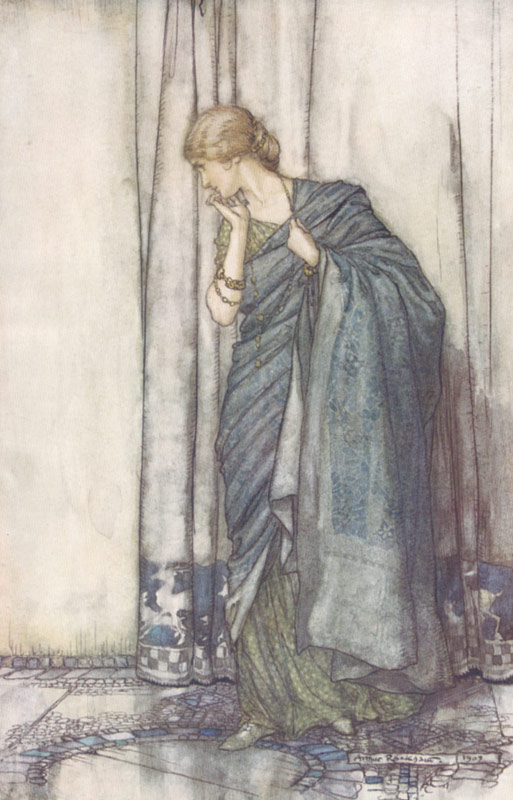
\includegraphics[width=2in]{media/image1.jpeg}
\caption{Helena Listening by Arthur Rackham}
\end{center}
\end{figure}

If you're playing an RPG solo it seems like there can be no
secrets. Take the simplest of situations in a solo game: you arrive at a
door. Maybe the scenario description says there is a 50\% chance of there being something
behind the door. You roll percentile dice to see what happens as you
open it. In a weak sense there was a secret: you didn't know there
was a dragon behind the door before you opened it. But if you were
playing with a GM you could do more -- you could listen at the door
first in order to find
out if there was anything behind it.

\begin{figure}
\label{tree1}
\begin{center}
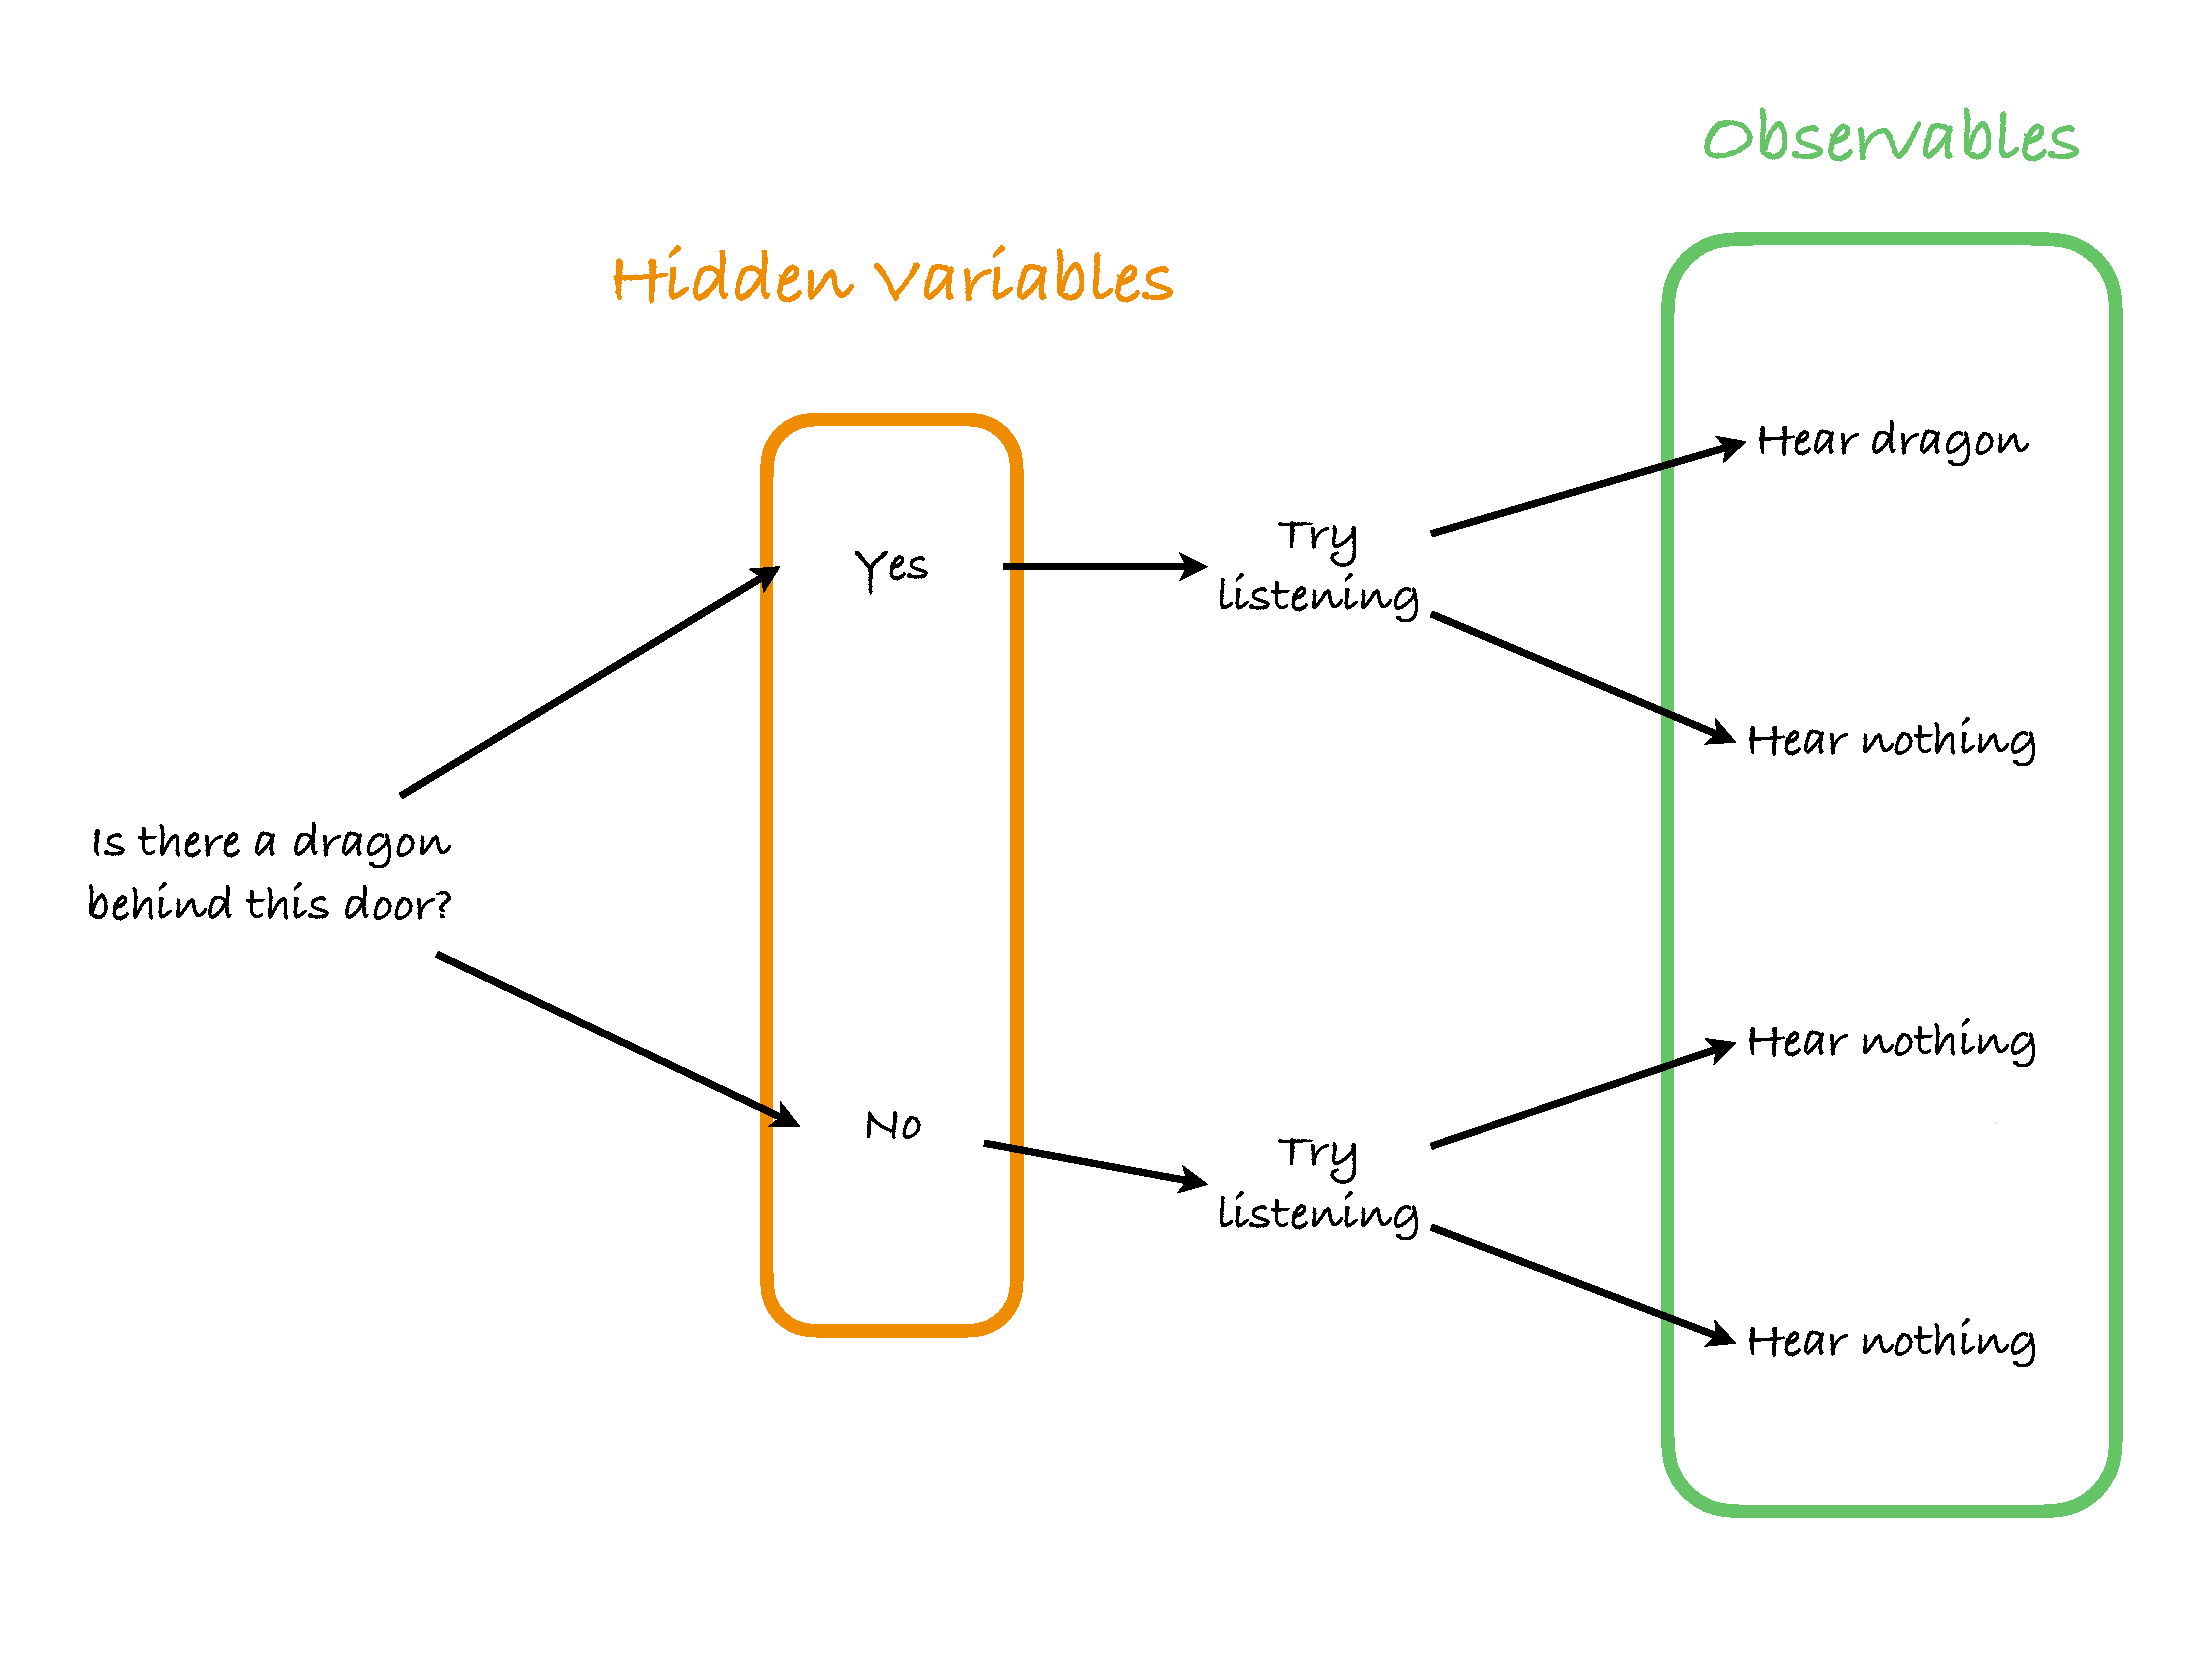
\includegraphics[width=5in]{media/Tree1.pdf}
\caption{The mechanics of listening at a door}
\end{center}
\end{figure}

Let's say that if something
lies behind the door then you have a 50\% chance of hearing it, but when
roll to listen you hear nothing. Maybe there is nothing there. But maybe
there's a dragon and you just didn't hear it. The GM can keep
you in suspense. They are able to keep a secret about what's behind the
door, and by listening you learn something about their secret.
But when playing solo you can't simulate
this. It's hard to simulate give yourself clues about something
you aren't supposed to know.

Except you can! For one thing, there's a standard ``textbook'' approach
we could take. We're not going to take it but for completeness I think I
ought to sketch it. It goes like this:
assuming the 50\%'s I hypothesised above, we can use Bayes' theorem
to compute that if you listen at the door and hear nothing then there's
now a 1/3 chance of there being something there. So you could roll for
this new probability. The outcome is, probabilistically speaking, the
same as if a GM was present using their knowledge of what is lurking
there. But nobody wants to use theorems to compute probabilities during
a game (do they?), and even if they could, the resulting probabilities
are likely to be tricky to roll for. In the example above we started
with percentiles (50\%'s in fact) and yet we need a 1/3 probability
which is awkward using percentile dice.

The alternative I propose is using the dice to do the calculations for
us. Not only can we do this but we can do it in a way that's not all
that weird, once you get used to it.

\hypertarget{hidden-variables-and-observables}{%
\section{Hidden variables and observables}\label{hidden-variables-and-observables}}

In any scenario there are the \emph{hidden variables}, things we're not sure
of, like whether or not there is a dragon behind the door. And there are
\emph{observables}, things we know for sure, like what we hear or what we see
when we finally open the door. What typically happens in a game is that
a GM comes prepared with some hidden facts, or generates some facts randomly
and keeps them secret from you. Those are the hidden variables, and
based on those hidden facts (and some die rolls) the GM describes some
observations. The problem is
that in order to generate the observations in a solo situation we seem
to need to know the hidden variables.

The approach we take here starts ordinarily enough: you play the scenario
generating the hidden variables as usual so that you can generate the
observations. Observations are considered fixed and unchanging. If you
heard a noise, you heard a noise. But after the observations are
generated, any hidden variables you generated are considered ephemeral
and are discarded. Whatever values they took, these are not the values
that will be used going forward. Only the observations remain. If at
some future point you need to make another observation based on those
hidden variables you're going to generate new values for them -- and
do so with the correct probabilities, taking into account the
observations you made.
Knowing the value of a hidden
variable is of no use to you because any time you make a decision based on your
apparent knowledge of a hidden variable it's going to be replaced
with a new roll. And, maybe surprisingly, there's a straightforward
scheme for getting the same probabilities that you'd get with a GM.
This makes it possible to collect clues about something despite not
knowing everything about it.

\subsection*{The system}
Here is the system: if you want to make an observation of something new,
generate all the hidden variables in the usual way as if you were the GM,
and then generate
the observations. For example, roll to see if a dragon is behind the
door, and then roll to see if your listening skills reveal something.
If you
do hear something (or not), that's it, that's the observation you
make. But the hidden variable does not tell you if the dragon is
present. It might or might not be. That information is discarded. You
only use the observable outcome from this pair of rolls: the sound you
heard.
\iffalse
\begin{figure}
\begin{center}
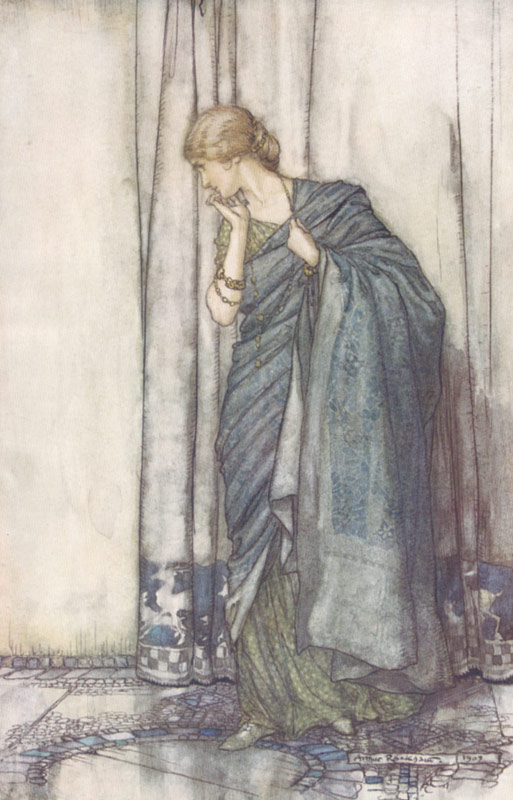
\includegraphics[width=1.67695in,height=2.65748in]{media/image1.png}
\end{center}
\end{figure}
\fi

Now suppose you want to make a second observation -- eg, opening the door
and actually looking.
Generate the hidden
variables again, and now roll \emph{again} for the \emph{first}
observation you made. This may sound weird, rerolling for something in
the past. But that makes the mathematics work out. When you reroll, if
the observation is consistent with what happened before (eg. in this
example, you hear nothing again), you can uswe the hidden variable and
go on with the second
observation, using its outcome.
If you get an inconsistency you start
rolling again from the beginning, generating a new hidden variable.
Keep doing this until
you achieve consistency, and then make the new observation based on
whatever hidden variables you just generated.

The rerolling, with its possible rejections,
is what
biases the odds to match what would happen if a GM was keeping track of
the hidden variables.

See Figure~\ref{tree1} showing two possible outcomes, but four different ways
of getting there.
Suppose we hear nothing, then the situation is now like in Figure~\ref{tree2}
with only three possibilities.
To generate new hidden variables consistent with what we heard before
we need to generate the hidden variables in a way that makes the dragon less likely.
We follow the same tree again but reroll if we end up on the disallowed
branch. The presence, or not, of the dragon, will have the correct
probability.

\begin{figure}
\label{tree2}
\begin{center}
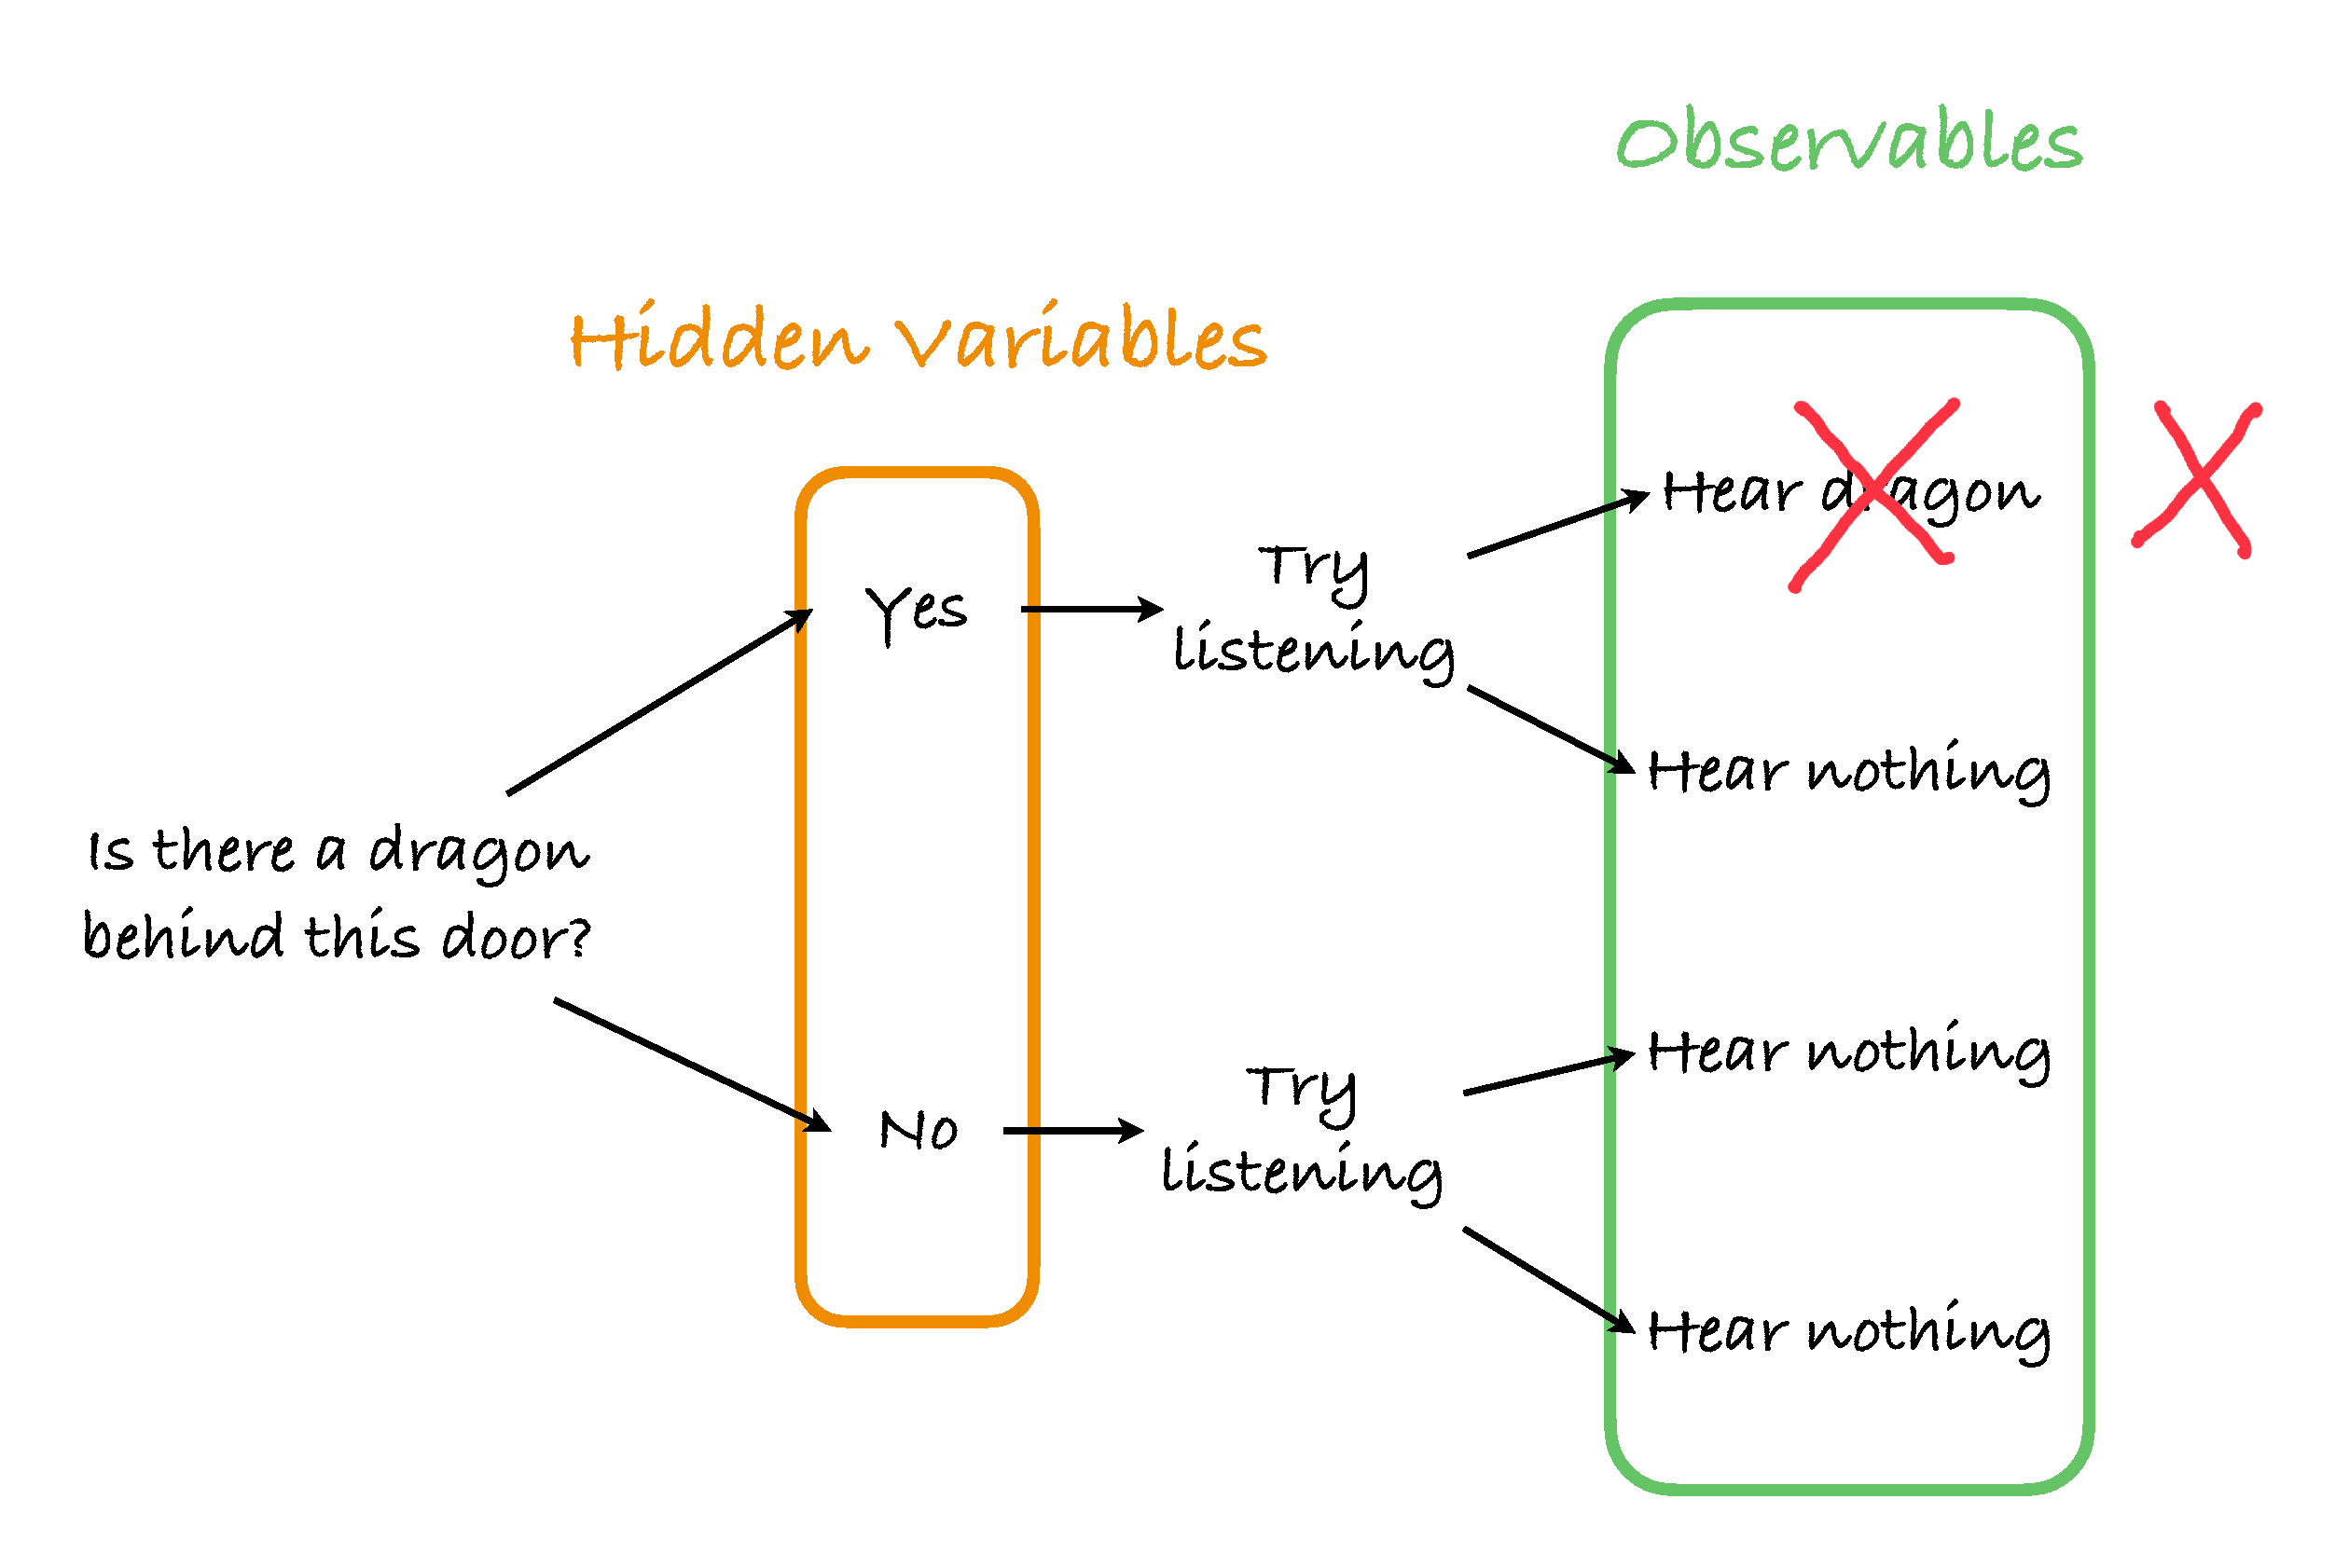
\includegraphics[width=5in]{media/Tree2.pdf}
\caption{If we heard nothing, then to get the correct probability of there
being a dragon we need to reject outcomes that lead to hearing something.}
\end{center}
\end{figure}

Let's try the door listening example with real rolls to illustrate
the process. And I'll do it a few times just to illustrate the
variations. (And I've put many more examples the appendices.) I'll use
\textbf{bold} for the individual rolls and \emph{italic} for actual
observed outcomes.

\subsubsection*{Listening once and opening door}

Let's say there's a 45\% chance of a dragon behind the door
and that if you listen at a door you have a 65\% chance of hearing
whatever is there.

\begin{quote}
\emph{Simulation 1}

I arrive at the door and listen. So I generate the hidden variable. I
roll \textbf{19}. So we pretend there is something behind the door. Now
I try to listen. I roll \textbf{58}. \emph{I hear something}. Well
that's that, I know for sure there is something behind the door.

\hrulefill

\emph{Simulation 2}

I arrive and listen. I roll \textbf{43}, so (temporarily) something is
present. I try to listen and get \textbf{78} which means \emph{I hear
nothing}. It's important to understand that the observation ``I hear
nothing'' is fixed, but that roll of 43 does not mean something will be
present when I open the door. Feeling confident, I now open the door. So
again, I roll to see if the monster is present and get \textbf{87}.
This is consistent with hearing nothing.
\emph{There is no monster}.
\end{quote}

There are lots more examples of this scenario in Appendix A.

\subsubsection*{Listening twice and opening door}

Let's try again but with rules that allow two attempts at
listening.

\begin{quote}
\emph{Simulation 1}

We're going to make our first listening attempt. First the hidden
variable, is there a monster behind the door? \textbf{90}. The hidden
variables is ``no monster''. We don't even need to roll for the
first attempt at listening. We know \emph{we hear silence on the first
attempt}.

Now we decide to listen again. Reroll for dragon presence: \textbf{22}.
Maybe, but reroll the listen: \textbf{32}. That's inconsistent with
our first attempt.

Restart the process: is dragon present?
\textbf{33}. Yes. Listen: \textbf{85}. Silent. That's compatible.
So we can now roll for the second listen: \textbf{41}. Our final
observation is that \emph{we hear the dragon on the second attempt} -
and obviously, if we heard it, it'll be there when we open the door.

\hrulefill

\emph{Simulation 2}

Is dragon there? \textbf{94}. No. So \emph{first attempt at listening
gives silence}. Listen again. Reroll for dragon: \textbf{20}. Present.
Reroll first listen: \textbf{85}. Silence,
consistent, so now roll for second listen: \textbf{24}. \emph{Final
observation: we hear the dragon!}
\end{quote}

See Appendix B for more examples of this scenario.

\iffalse
\subsubsection{The treasure is in one of four chests}

Now let's try a different scenario. There are four chests. Three
have (non-magical) traps. One contains a magic item. You don't know
which is which. You can cast two detect magic spells. They each have a
50\% chance of working.

\begin{quote}
\emph{Simulation 1}

Cast detect magic on first chest. First determine the hidden variable
for location of treasure: \textbf{4}. So \emph{detect magic on first
chest is going to say no and that's our first observation}. Now try
second chest: reroll for location \textbf{2}, now try detect magic:
\textbf{91}. \emph{We detect nothing on second attempt}. So let's
open third chest: reroll for location \textbf{3}. \emph{We open it and
get the treasure!}

\emph{Simulation 2}

Cast detect magic on first chest. Determine location of treasure first:
\textbf{4}. So \emph{we detect nothing}.

Cast detect magic on same chest: reroll location \textbf{1}. Detect
magic: \textbf{82}. So \emph{no magic detected on second try}.

So let's open it: reroll location \textbf{2}. So \emph{opening
chest 1 reveals a trap}. Ouch! That was stupid.

Anyway, you survive so let's open chest 2. Reroll location
\textbf{4}. That's consistent with what we know. \emph{Again, it's
not the treasure}. Ouch, more damage.

Ok, on to chest 3. Roll for location and we roll \textbf{3}. Woo hoo,
\emph{after two lots of damage we get the treasure}.
\end{quote}

See Appendix C for more examples of this scenario.

\hypertarget{optimisations}{%
\section{Optimisations}\label{optimisations}}

There are some optimizations we could use.
A player should never
make a decision based on hidden variables. Whenever there is a decision
point you need to start generating hidden variables again. But if you
commit to a course of action then it's safe to keep using a hidden
variable as you're obviously not making use of it.
Eg. if you
promise (to yourself) to first perform detect magic on chest 1 and then,
if nothing is detected, to perform it on chest 2,
then you don't need to reroll for the
location of the treasure between the detect magic spells.
But you need
to not cheat and bail out if something doesn't go your way.

Also note that if you've already opened 2 chests, you can use d2
to determine the hidden variables for the location of the treasure when
you investigate the third chest.

It's probably worth writing down the observations that are made as
these are the things that need to be rerolled consistently.
And notice
how I elided many rolls. Eg. if the hidden variable says there is
nothing behind the door then you don't have to actually do the
listen roll. But note that even if you don't do the roll you need to
consume any consumable resources associated to the action -- like maybe
your scroll turns to dust. This means that sometimes you'll make
fewer rolls than if you were working with the GM because the GM
sometimes has to make you roll even when the outcome is a foregone
conclusion for them.

Because the chest example takes a few rolls, that's probably a
reasonable upper bound on the complexity that a player could tolerate.

\hypertarget{more-scenarios}{%
\section{More Scenarios}\label{more-scenarios}}

\emph{Illusions}

You're fighting a single monster but you know it has a 50\% chance
of being an illusion. Any time an illusion hits you, you believe
it's real and take damage. But any time you hit an illusion it is
dispelled. This scenario is straightforward to play. When you first hit,
you roll the percentile dice to check whether it's an illusion.
Once you've hit there is nothing more to be revealed.

Suppose you attack many monsters and each one has an independent chance
of being an illusion. We can just play this out with each individual
monster working just like a single monster -- checking whether or
it's an illusion on the first hit.

A more interesting case is a single monster that can project, say, three
illusions of itself while fighting. Now the probabilities are no longer
independent as we know there is precisely one real monster. In this
case, the first time you hit one of the four you roll d4 to see which is
the illusion. If you hit the real monster then there is nothing more
hidden. Otherwise it is dispelled and now only one of three is real.
Next time you hit you roll d3 to determine which is the real monster and
so on.

\emph{Unknown hit point battle}

It can be reasonable to simulate fighting a monster with an unknown
number of hit points, depending on how the HP were generated. Let's say
it has d8 HP. We don't generate the HP until we first hit it. Let's say
we do 3 damage. Now we roll the d8 for its HP. If we get 1-3, the
monster is dead. If we get 4-8 the monster is still alive. But we don't
record the actual value of the HP. Instead we record that it has 1-5 HP
left. Next time we hit we can use d5 to determine its hit points and so
on. But, this only works so easily. because if we use d8 to generate its
hit points then all values from 1 to 8 are equally likely. If, instead,
we use 2d6 for HP, then the values from 2 to 12 aren't equally likely.
Let's play out an example showing how to handle this case:

\begin{quote}
\emph{Simulation 1}

You attack the monster and do \textbf{5} damage. Now you must roll for
its HP. Let's say we get \textbf{8}. So we know \emph{the monster
survives}. We don't record the 8. Instead we record that the monster
started with 6-12 HP. Now we hit again and do \textbf{3} more damage. We
need to determine its HP again. Keep rolling 2d6 until we get a
consistent value in the range 6-12. If we get 9 or more, let's say
\textbf{10}, \emph{the monster survives the second attack} and we note
its initial HP as being in the range 9-12. And so on\ldots{}
\end{quote}

\emph{Placebo or healing potion}

A possible scenario is a healing potion that restores 1d6 hit points but
you don't know how many. (How many times have you taken a painkiller and
not felt any different?) This isn't very different from the situation of
fighting a monster with unknown hit points except now we have a player
with d6+N hit points where N is the number if the potion hadn't been
consumed. Remember the potion restores HP but can't give you more than
you started with.

\begin{quote}
\emph{Simulation}

The player started with 8HP, had their HP reduced to 4, then sipped a
healing potion restoring 1d6 and subsequently took 1HP more damage. So
they currently have 3+1d6 HP with 7 and above treated as 7 (because of
that extra 1HP damage). Now they are struck with a blow doing 5 HP
damage. Roll for the healing value of the potion. Let's say it's
\textbf{3}. The player survives and we have the observation that
\emph{the player had 6 or more hit points when hit and that the potion
must have healed them by 3 or more HP}. In effect, the player now has
1d4 HP but with a maximum of 2.

That needed quite a bit of reasoning, but we can make it easier.

We start by writing down the player's HP: 8.

They get their HP reduced to 4.

They take the potion. Now write their HP as 5 6 7 8 8 8.

After that extra 1HP of damage it becomes 4 5 6 7 7 7

Now comes that 5HP blow. We are left with -1 0 1 2 2 2

We roll d6 to determine the hidden variable for the potion restoration.
In the example above we got 3. The third value is 1, so we survive, and
now we are left with the four possibilities 1 2 2 2, all equally likely.
Next time we want to determine the hidden variables for our HP we can
roll d4.
\end{quote}
\fi
\hypertarget{design-considerations}{%
\section{Design Considerations}\label{design-considerations}}

The question now is how to design scenarios with these new possibilities
in mind.
We can now allow solo players to make strategic use of things
like detection abilities.
These can add to the
fun and also the sense of agency -- you feel like you're making decisions
based on evidence.

Here are some examples I've tested:
\begin{enumerate}
\item multiple treasure chests, all but one with a trap,
one with a magic item, and the player has a detect magic scroll.
\item a healing potion that has a 50\% chance of having worked
but the player doesn't know for sure.
(Can you always feel the difference if you just took an ibuprofen?)
\item Fighting monsters (like the D\&D one based on van Vogt's Black Destroyer) that generate illusions
that are dispelled on the first hit.
\item Fighting monsters with an unknown number of hit points(!)
\end{enumerate}

But things can get messy.
For example, we could have a potion that restores an unknown
number of hit points determined by d6.
This is perfectly playable but it might require frequently regenerating the hidden d6
and, this might not be obvious at first, checking the player's entire
HP history
each time there is the possibility of being reduced to zero hit points.
And what if there are two such potions available?
It gets really messy.
So scenarios need to be designed in such a way that multiple hidden variables don't
interact.

The probabilities ought to be near the middle of the range -- 50\%.
If not, you run the risk that you will have to reroll many times to reproduce
a consistent history.
This could be pretty unpleasant when fighting monsters with an unknown number of hit points
so I really wouldn't use that example!

I would just use this technique in occasional places of special interest
rather than everywhere.
And I'd probably mostly stick with simple detection scenarios, especially if
a scenario is distributed a s a self-contained unit with all of its rules.

But not that I've described some of these more complex scenarios as some of them
can be made much more playable by the use suitable player aids.
I leave their design as an exercise.

\iffalse
If
we allow players two opportunities to acquire a 1d6 healing potion then
the health restored is 2-12, but these aren't equally likely outcomes
which prevents us from using the optimization I described for when all
outcomes are equally likely. This puts a heavy burden on a player.

So in general you want to try to make hidden variables independent from
each other. Have rules that say you can only listen once, have only one
detect magic scroll available, only one health potion available and so
on. You need to anticipate possibilities too. Fighting individual
monsters with unknown numbers of HP is fine, but what happens if a
player can use a charm spell to make one monster with unknown HP fight
another. It can start to get hairy.

It's also possible, if they're unlucky, that a player might find
themselves rolling again and again in order to get rolls consistent with
previous observations. The simplest rule of thumb I can come up with to
avoid this is to design scenarios that tend to involve probabilities
that don't stray too far from 50\%. If listing at a door has a 99\%
chance of success, and you're unlucky enough to fail on the first
listen, then on rerolls you have to reproduce that 1\% chance of
failing. That could get annoying quickly!

This isn't something I'd use everywhere in a scenario. I like the
detection scenarios, like maybe a small number of one shot detect
monster scrolls. Maybe one monster with unknown HP. The illusion case is
easy to handle.
\fi

\hypertarget{mathematical-notes}{
\section{Mathematical notes}}
\label{mathematical-notes}

The method I describe here is essentially a form of \href{https://en.wikipedia.org/wiki/Rejection_sampling}{rejection sampling}.

It's also reminiscent of a technique used for something in computer
science called \emph{consistent distributed hashing} described in
\href{https://arxiv.org/abs/1406.2294}{{\em A Fast, Minimal Memory, Consistent Hash Algorithm}}.

In essence, for reasons of fairness, you
assign certain responsibilities to computers in a network by throwing
darts at a dartboard.
But as time goes by you need to shift
responsibilities by redrawing the lines around the darts and noting
which regions the darts end up in. Lamping and Veach\footnote{
  Veach invented the original auction method used by Google to allow advertisers to bid
  for having their ads appear according to what keywords you type. He
  also invented a crucially important method to render glossy surfaces
  in 3D graphics.} came up with a trick involving not bothering to
retain the position of the dart, just what region it was in, and
arranging that the probability of it changing region is the same as if
your policy was to track the exact dart positions.

I also want to mention \href{https://arxiv.org/abs/1710.10385}{{\em Capturing the Future by Replaying the Past}}
by Koppel at al.
It's about the idea that sometimes you want a computer program to continue
from an earlier state but that facility isn't available to you so instead
you start again from the beginning.
(Reminiscent of video games in the old days.)
That's what we're doing here and the similarity is more than superficial.

\hypertarget{final-word}{%
\section{Final word}\label{final-word}}

\begin{quote}
Reports that say that something hasn't happened are always interesting
to me, because as we know, there are known knowns; there are things we
know we know. We also know there are known unknowns; that is to say we
know there are some things we do not know. But there are also unknown
unknowns---the ones we don't know we don't know.

Donald Rumsfeld, 2002
\end{quote}

The observables correspond to known knowns and the hidden variables are the known
unknowns. But I've nothing to say about unknown unknowns.

\section{Appendices}

\hypertarget{appendix-a}{%
\subsection*{Appendix A}\label{appendix-a}}

\subsubsection*{More examples of listening once and opening door}

\begin{quote}
\emph{Simulation 3}

Arrive and listen. Roll to see if Dragon is there: \textbf{50}. There's
no need to bother with the listening roll, as \emph{nothing is heard}.
But we still can't take this as meaning there is no dragon because
the presence of the dragon is a hidden variable.

Let's open the door. Roll to see if the monster is present:
\textbf{47}. Just misses 45, and it's not. Trying to listen now
would give no sound, consistent with the previous roll, so we can accept
that 47 as saying \emph{the dragon is absent when we open the door}.

\hrulefill

\emph{Simulation 4}

Arrive. Listen. Roll to see if the dragon is there? \textbf{06}. The
hidden variable says yes. Now roll to listen: \textbf{41}. \emph{You
hear something. We know the dragon is there!} As this is an actual
observation we know it will actually be there when the door is opened.

\hrulefill

\emph{Simulation 5}

Arrive. Is Dragon there? \textbf{26}. Yes. Try listening: \textbf{90}.
Hear nothing\emph{.} So the actual observation is that \emph{you hear
nothing}.

Now we open open door. Reroll for dragon presence: \textbf{09}. Now we
need to reroll for listening: \textbf{96}. We hear nothing. That's
consistent with the previous roll. So we have to accept that 09 as
meaning \emph{the dragon is there} despite not hearing it. Ouch!
Important note: you're not allowed to bail out after rerolling for
the dragon presence.
That's called cheating.

\hrulefill

\emph{Simulation 6}

Arrive. Is Dragon there? \textbf{44}. The hidden variables says yes.
Listen: \textbf{08}. Yes, \emph{you observe it is there}.

\hrulefill

\emph{Simulation 7}

Is the Dragon there? \textbf{56}. No. Try listening: \textbf{88}. The
actual observation is to \emph{hear nothing}.

Now open the door. Reroll for dragon presence: \textbf{41}. It's
there (as a hidden variable), but reroll for listening: \textbf{37}. So
you hear it. But that's inconsistent with before. Roll again for
dragon presence: \textbf{72}. It's not there. No need to roll for
listening again as the outcome will be silence. So we can take that 72
as meaning \emph{there is no dragon observed behind the door}.
\end{quote}

Note how in my seven trials, the worst case required 5 rolls. It's
theoretically possible that you could keep rolling for a long time -
because when you first listen you hear nothing but every resimulation
says a dragon is present and you hear it, forcing a reroll. But
that's extremely unlikely.
\iffalse And we could have saved several rolls by
switching to d3 when there were only three chests left and d2 when there
were just two.
\fi

\hypertarget{appendix-b}{%
\subsection*{Appendix B}\label{appendix-b}}
\subsubsection*{More examples of listening twice and opening door}

\begin{quote}
\emph{Simulation 3}

Is the dragon there? \textbf{79}, no. \emph{So listening gives silence}.
Of course the dragon might be there when we open the door.

Listen again, rerolling for the presence of the dragon: \textbf{24},
it's present. Reroll first listening attempt: \textbf{76} silence.
Consistent. Now roll second listen: \textbf{81}, silence. After
\emph{hearing silence twice} you choose to enter.

Again, roll for dragon: \textbf{56}, not present. We know that listening
will give silence twice so this is consistent with previous
observations. So we accept 56 as meaning there is no dragon when we open
the door. That took 5 rolls.

\hrulefill

\emph{Simulation 4}

Is dragon there? \textbf{43}. Yes. Listen: \textbf{49}. \emph{We hear it
first time} so that ends our observations.

\hrulefill

\emph{Simulation 5}

Is dragon there? \textbf{62}, no dragon. \emph{Listening first time
gives silence}.

We choose to listen again: reroll for dragon: \textbf{88}, no dragon so
\emph{we hear silence second time too}.

Now open door. Reroll for dragon: \textbf{29}, it's there (in the hidden
variable). Reroll first time listening: \textbf{33}. We hear it.
Inconsistent.

Reroll for dragon: \textbf{46}. This means we get silence twice and we
can take the 46 as meaning there really was \emph{no dragon}.

\hrulefill

\emph{Simulation 6}

\textbf{37} dragon may be present. Listen: \textbf{20} so \emph{you hear
it first time!}

\hrulefill

\emph{Simulation 7}

\textbf{92} no dragon present so \emph{first listen gives silence}.

Listen again so reroll for dragon: \textbf{73} and \emph{silence again}.

Now open door: reroll for dragon: \textbf{22}, so maybe present, reroll
first listen: \textbf{87} silence, consistent with before. Reroll second
listen: \textbf{98}, silence again, so now we can accept the 22 as
meaning \emph{the dragon really was present} despite the fact that we
got silence twice! Bad luck.
\end{quote}
That last simulation took 5 rolls. If a GM was present it would have
been just 3 rolls.

\iffalse
\hypertarget{appendix-c}{%
\subsubsection{Appendix C}\label{appendix-c}}

\begin{quote}
\emph{Simulation 3}

Cast detect magic on first chest, so roll for location of treasure:
\textbf{2}. So \emph{no magic detected}.

Cast detect magic on chest 2. Roll for location: \textbf{2} (again).
Roll to detect magic: \textbf{25}. So \emph{the item is found!}

Simulation 4

Cast detect magic on first chest, roll location: \textbf{1}. Detect
magic: \textbf{44}. Magic detected. That one was too easy.

\emph{Simulation 5}

Cast detect on first chest. Roll for location: \textbf{2}. \emph{No
magic detected}.

Detect on second chest: location roll: \textbf{3}, so no magic detected.

So open chest 3. Reroll location: \textbf{4}. Bang! \emph{Trap
triggered}.

But still alive so open chest 4. Reroll location: \textbf{3}.
That's inconsistent.

Try again: reroll location: \textbf{1}. Now reroll the first detect:
\textbf{41}. Not consistent.

Reroll location: \textbf{3}. Inconsistent.

Reroll location \textbf{3}. Still inconsistent.

Reroll location: \textbf{1}. Reroll detect: \textbf{56}. No magic
detected. That's also consistent with not detecting magic the
second time. So we can accept 1 as the location for the purposes of
deciding what's in chest 4. \emph{Ow ow}!

Now open chest 1. Reroll location: \textbf{2}. We did a detect magic
there so reroll that: \textbf{16}. That's incompatible.

Reroll location: \textbf{4}. We know it's not there.

Reroll location: \textbf{4}.

Reroll location: \textbf{4}. Are these dice faulty? I used real rolls to
write this.

Reroll location: \textbf{1}. Reroll detect: \textbf{44}. Inconsistent.

Reroll location: \textbf{3}. Inconsistent.

Reroll location: \textbf{1}. Reroll detect: \textbf{82}. Nothing
detected. That's consistent with what actually happened. So we can
take 1 as the location and \emph{we get the treasure after triggering
two traps}. That took 20 rolls. But a lot happened: detect magic was
cast twice and 3 chests were opened.
\end{quote}

\hypertarget{references}{%
\subsubsection{References}\label{references}}

https://en.wikipedia.org/wiki/Rejection\_sampling

\href{https://arxiv.org/abs/1406.2294}{{A Fast, Minimal Memory,
Consistent Hash Algorithm, John Lamping, Eric Veach}}\\
This paper has a neat trick that is similar to the method of trac king
ranges I described in the fight with unknown hit points

\hypertarget{image-credits}{%
\subsubsection{Image Credits}\label{image-credits}}

\begin{enumerate}
\def\labelenumi{\arabic{enumi}.}
\item
  \emph{Helena Listening} by Arthur Rackham
\item
  Polyhedral dice image:
  \href{https://commons.wikimedia.org/wiki/File:Des_polyedriques.svg}{{https://commons.wikimedia.org/wiki/File:Des \_polyedriques.svg}}
\end{enumerate}
\fi

\end{document}